\section{Creating a forked local repository\label{sec:local_repo}}
This section will cover the following points
\begin{enumerate}
	\item Create a github profile
	\item Download git software
	\item Fork the master repository
\end{enumerate}


\subsection{Git Profile}
The first step you will have to do is create a profile on github (if you do not already have one). Github is free and easy to setup. Go to \url{https://github.com} to set up a profile if you do not already have one. Once you have set up a github account you need download git software that you use to "communicate" to repositories.


\subsection{Git Software}
As mentioned earlier the source code is hosted on github so before you can get a copy of the repository you will need to install a program that can "communicate" with github. You will need to acquire Command line GIT from \url{https://git-scm.com/downloads} this is because it is used to build a Version.h header file so \CNAME\ but this will be discussed earlier. I use tortoisegit \url{https://tortoisegit.org/download} on windows to pull, push and commit changes to repositories. However there are many programs to use and all have the same functionality.

\subsection{Forking a repository}

The main repository which contains code that is in the publicly available \CNAME\ executable is called the 'master' repository. Only the development team have permission to add, delete and change code directly with the 'master' repository. For other contributors there is a very easy way to add, delete and change code. This is through forking the master repository. This is done by going to the \CNAME\ github repository found at \url{https://github.com/NIWAFisheriesModelling/CASAL2} and selecting the fork button in the top right of the page circled in Figure~\ref{fig:fork}

\begin{figure}[!ht]
	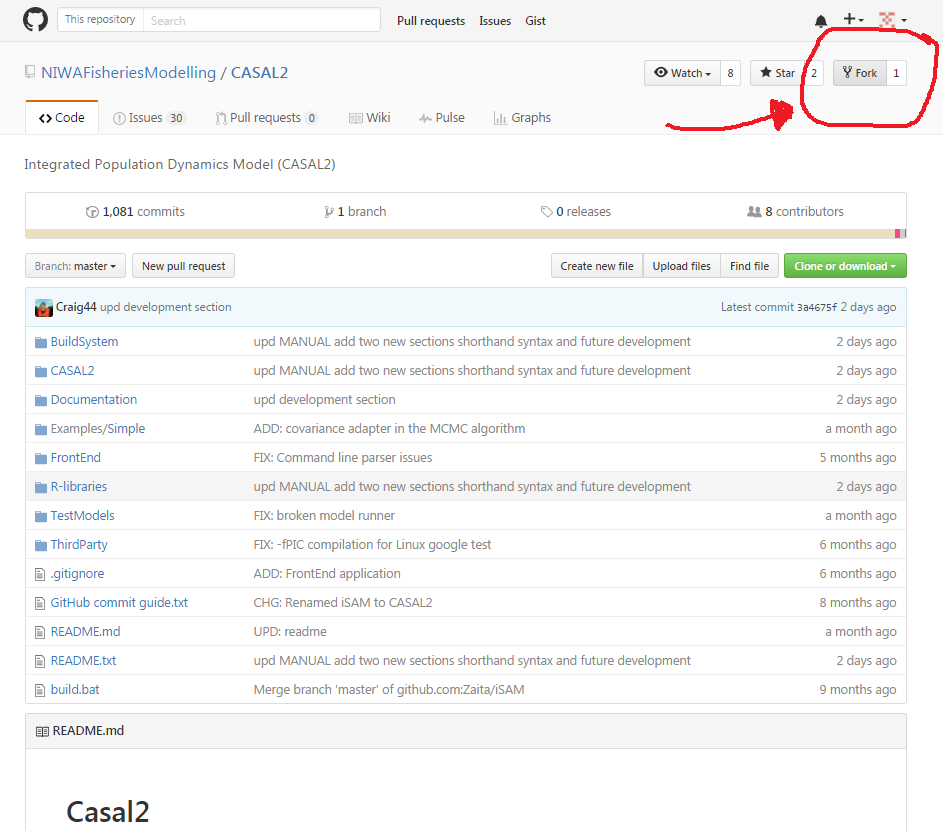
\includegraphics[scale=0.6]{Figures/Fork_button.png}
	\caption{Creating a forked repository}\label{fig:fork}
\end{figure}
\pagebreak
This will create a copy of the \CNAME\ repository under your profile at the point of the fork. To check that you have successfully forked the repository, go to your git profile and you should see a \CNAME\ repository under your repositories, shown in Figure~\ref{fig:fork_success},

\begin{figure}[!ht]
	\includegraphics[scale=0.6]{Figures/Fork_success.png}
	\caption{Fork success}\label{fig:fork_success}
\end{figure}

An important point is that the forked repository will not automatically keep up to date with the 'master' repository. So if the development team make changes, you will want to keep your forked repository up to date. This is easily done and is explained in the next section on how to maintain and contribute to a forked repository.


